
\subsection{Modelado}%
\label{sub:modelado}
En primer lugar, se definieron relaciones básicas de acuerdo a los requerimientos del sistema para poder crear las clases admin y definir las entidades como
recursos \textit{API-Platform}.

\subsubsection{Introducción a Doctrine}%
\label{ssub:introducción_doctrine}
Con Doctrine, cada objeto PHP que se requiera persistir a la base de datos, necesita estar definido en un archivo PHP que
contiene información referente a tipos de dato y relaciones entre entidades. A este archivo se lo denomina entidad.

\begin{figure}[H]
    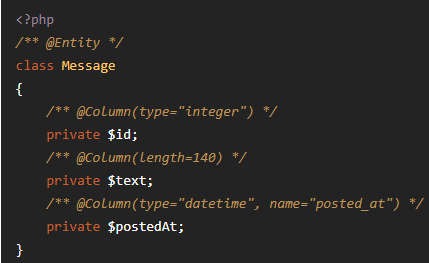
\includegraphics[width=1\linewidth]{image/entidad-doctrine.png}
    \caption[Ejemplo básico de una entidad]{Ejemplo básico de una entidad.\newline \textbf{Fuente:} Recuperado de \url{www.doctrine-project.org/
    projects/doctrine-orm/en/2.6/reference/basic-mapping.html}}%
    \label{fig:image/entidad-doctrine}
\end{figure}
Una relación en \textbf{Doctrine} está formado por dos entidades. Una de ellas actúa como el lado propietario de la relación y la otra como el inverso\@.
El lado propietario de la relación es aquel en el que \textbf{Doctrine} verifica si hubo cambios.
Existen dos tipos de mapeo de relaciones, bi-direccionales y uni-direccionales\@.
Una relación bi-direccional permite que ambos lados de la relación puedan accederse entre sí\@. En cambio, una relación uni-direccional sólo puede accederse
a través del lado propietario\@.
Al trabajar con relaciones, se debe tener en cuenta la manera en que Doctrine comprueba por cambios en los datos, ya que cambios persistidos en el lado
inverso de la relación serán ignorados por el ORM al momento de actualizar información a la base de datos.



\subsubsection{Actividad}%
\label{ssub:actividad}
Se modeló el siguiente esquema de acuerdo a la información recibida por parte del Área de Informática de la universidad\@.
Además, se pensó en utilizar herencia para la definición de las actividades, de esta manera cada cargo o actividad en particular
heredaría toda característica común de una entidad padre.

\begin{figure}[H]
    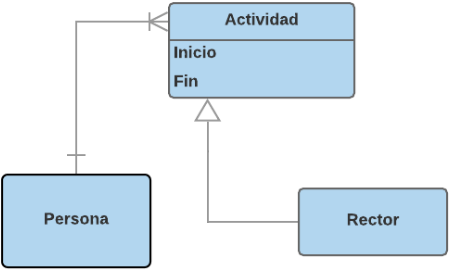
\includegraphics[scale=1]{image/actividad-modelo.png}
    \caption[Ejemplo de la definición de un cargo]{Ejemplo de la definición de un cargo.\newline \textbf{Fuente:} Elaboración propia}%
    \label{fig:image/actividad-modelo}
\end{figure}
El primer paso realizado para la definición de cada cargo o actividad fue la creación de la entidad \textit{Actividad}, la cual contendrá
datos de la persona relacionada y el periodo de desarrollo de la actividad o cargo\@.
Se agregó la función de Soft delete o borrado lógico, la que permite que, al borrar una actividad desde la aplicación web,
la misma es ocultada del usuario y no borrada de la base de datos\@. Esta función posibilita almacenar datos históricos del sistema\@.
Además, se agregó la función de Time stamps o etiquetas de tiempo, la cual hace posible el seguimiento de las fechas de creación
y actualización de cada actividad.


Se definió el mapeo de esta entidad en Doctrine mediante herencia de clase, una estrategia en la que cada clase en la jerarquía es mapeada a varias tablas:
la propia y las de todas las clases padre. La tabla de una clase hija es vinculada a la del padre a través de una clave foránea.

Doctrine implementa esta estrategia a través del uso de una columna denominada discriminator en la tabla más alta en la jerarquía\@. Esta es la mejor
manera de lograr consultas polimórficas con herencia de clase\@. \parencite{doctrine-inheritance}\\
\noindent
Esta columna identifica el tipo de entidad, por ejemplo: una
fila con un valor de ``director instituto'' significa que es una actividad del tipo DirectorInstituto\@.
Si no se provee el mapeo correspondiente, doctrine lo generará automáticamente utilizando el nombre de cada clase entidad en minúscula\@. \parencite{doctrine-inheritance}

\begin{figure}[H]
    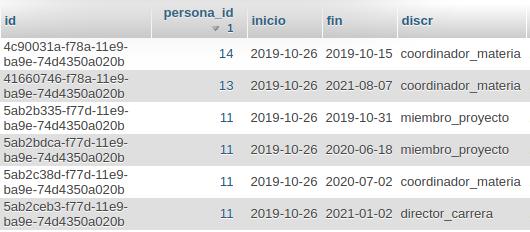
\includegraphics[width=1\linewidth]{image/discriminator-doctrine.png}
    \caption[Columna \textbf{discr} utilizada como discriminator]{Columna \textbf{discr} utilizada como discriminator.\newline \textbf{Fuente:} Elaboración propia, impresión de pantalla del código fuente.}
    \label{fig:image/discriminator-doctrine.png}
\end{figure}
\newpage
Se agregó la correspondiente metadata de la herencia en \textit{Actividad} y se optó por proporcionar el mapeo de la columna discriminator:

\begin{figure}[h]
    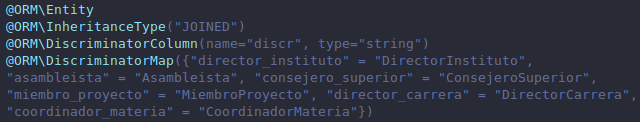
\includegraphics[width=1\linewidth]{image/discr.png}
    \caption[Mapeo de la columna \textbf{discriminator}]{Mapeo de la columna \textbf{discriminator}.\newline \textbf{Fuente:} Elaboración propia, impresión de pantalla del código fuente.}
    \label{fig:image/discr.png}
\end{figure}

\subsubsection{Miembro de Proyecto}%
\label{ssub:miembro_de_proyecto_modelo}
Esta entidad es la que almacenará datos acerca de la acción de formar parte de un proyecto. Cada dato de la columna \textbf{MiembroProyecto} representará la participación
de una persona a un proyecto\@.
Se mapeó la relación entre \textit{miembros} y \textit{proyectos} con una cardinalidad de 1-n y, dado que en este tipo de relaciones el lado n toma la clave foránea, el lado
propietario termina siendo \textit{miembros de proyecto}\@.
Con \textit{roles} sucede lo mismo, ya que cada instancia de miembro debe poseer un solo rol.

\begin{figure}[h]
    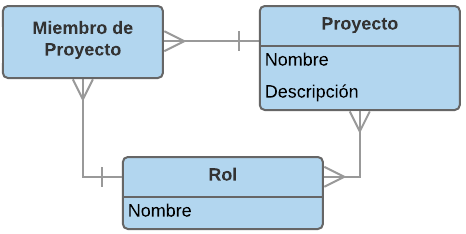
\includegraphics[width=1\linewidth]{image/mpr-new.png}
    \caption[Diagrama que representa la relación entre miembro, rol y proyecto]{Diagrama que representa la relación entre miembro, rol y proyecto.\newline \textbf{Fuente:} Elaboración propia utilizando una herramienta online de elaboración de diagramas.}
    \label{fig:image/mpr-new}
\end{figure}

\begin{figure}[h]
    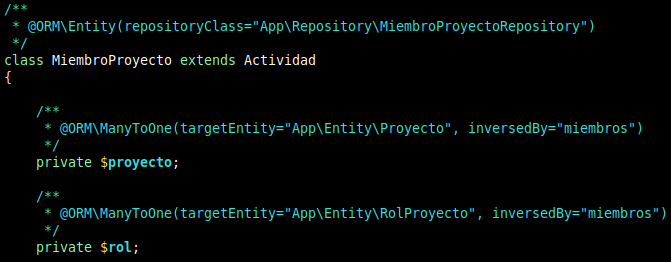
\includegraphics[width=1\linewidth]{image/miembros.png}
    \caption[Metadata de mapeo de relaciones de miembro de proyecto]{Metadata de mapeo de relaciones de miembro de proyecto.\newline \textbf{Fuente:} Elaboración propia.}
    \label{fig:image/miembros}
\end{figure}

\subsubsection{Proyecto}%
\label{ssub:modelo_proyecto}
En el sistema se necesita representar dos tipos de proyectos, de extensión y de investigación\@. Por ende, se decidió agregar \textbf{herencia} para la definición
de cada proyecto\@. Esto evita tener que crear una nueva entidad para representar los miembros del otro proyecto\@. De la misma forma que con Actividad se utilizó
herencia de clase.


En cuanto a sus relaciones, posee la relación con miembros desde el punto de vista de Proyecto. Con una cardinalidad de n-1 y siendo \textbf{Proyecto} el lado
inverso de la relación.

Por otro lado, también se definió su relación con \textbf{Roles de Proyecto} con una cardinalidad de n-n.

\subsubsection{Rol de Proyecto}%
\label{ssub:rol_de_proyecto_modelo}
Esta entidad representa un rol de proyecto, a cada instancia de miembro se le puede asignar un rol a ejercer en el Proyecto.

Se estableció la relación de roles del tipo n-n, es decir, con una cardinalidad de muchos a muchos; ya que un proyecto puede tener muchos roles y además
un rol puede tener muchos proyectos\@. Como la entidad de roles se actualizará a partir de los proyectos, se definió a Proyecto como dueño o propietario de
la relación. En el caso de una relación de este tipo el lado propietario es aquel que contiene el parámetro \textbf{inversedBy} en
su definición.~\parencite{doctrine-inheritance}
